\documentclass{standalone}

%----------------------------------------------------------------------------------------------%
%                                 Packages and basic declarations
%----------------------------------------------------------------------------------------------%

\usepackage{amsmath}
\usepackage{mathrsfs}
\usepackage{pgf}
\usepackage{tikz}
\usepackage{verbatim}


\usetikzlibrary{arrows}



%----------------------------------------------------------------------------------------------%
%----------------------------------------------------------------------------------------------%
%                                            DOCUMENT STARTS
%----------------------------------------------------------------------------------------------%
%----------------------------------------------------------------------------------------------%

\begin{document}

%----------------------------------------------------------------------------------------------%
%                Single RVE with applied constant strain, only debonded
%----------------------------------------------------------------------------------------------%
 
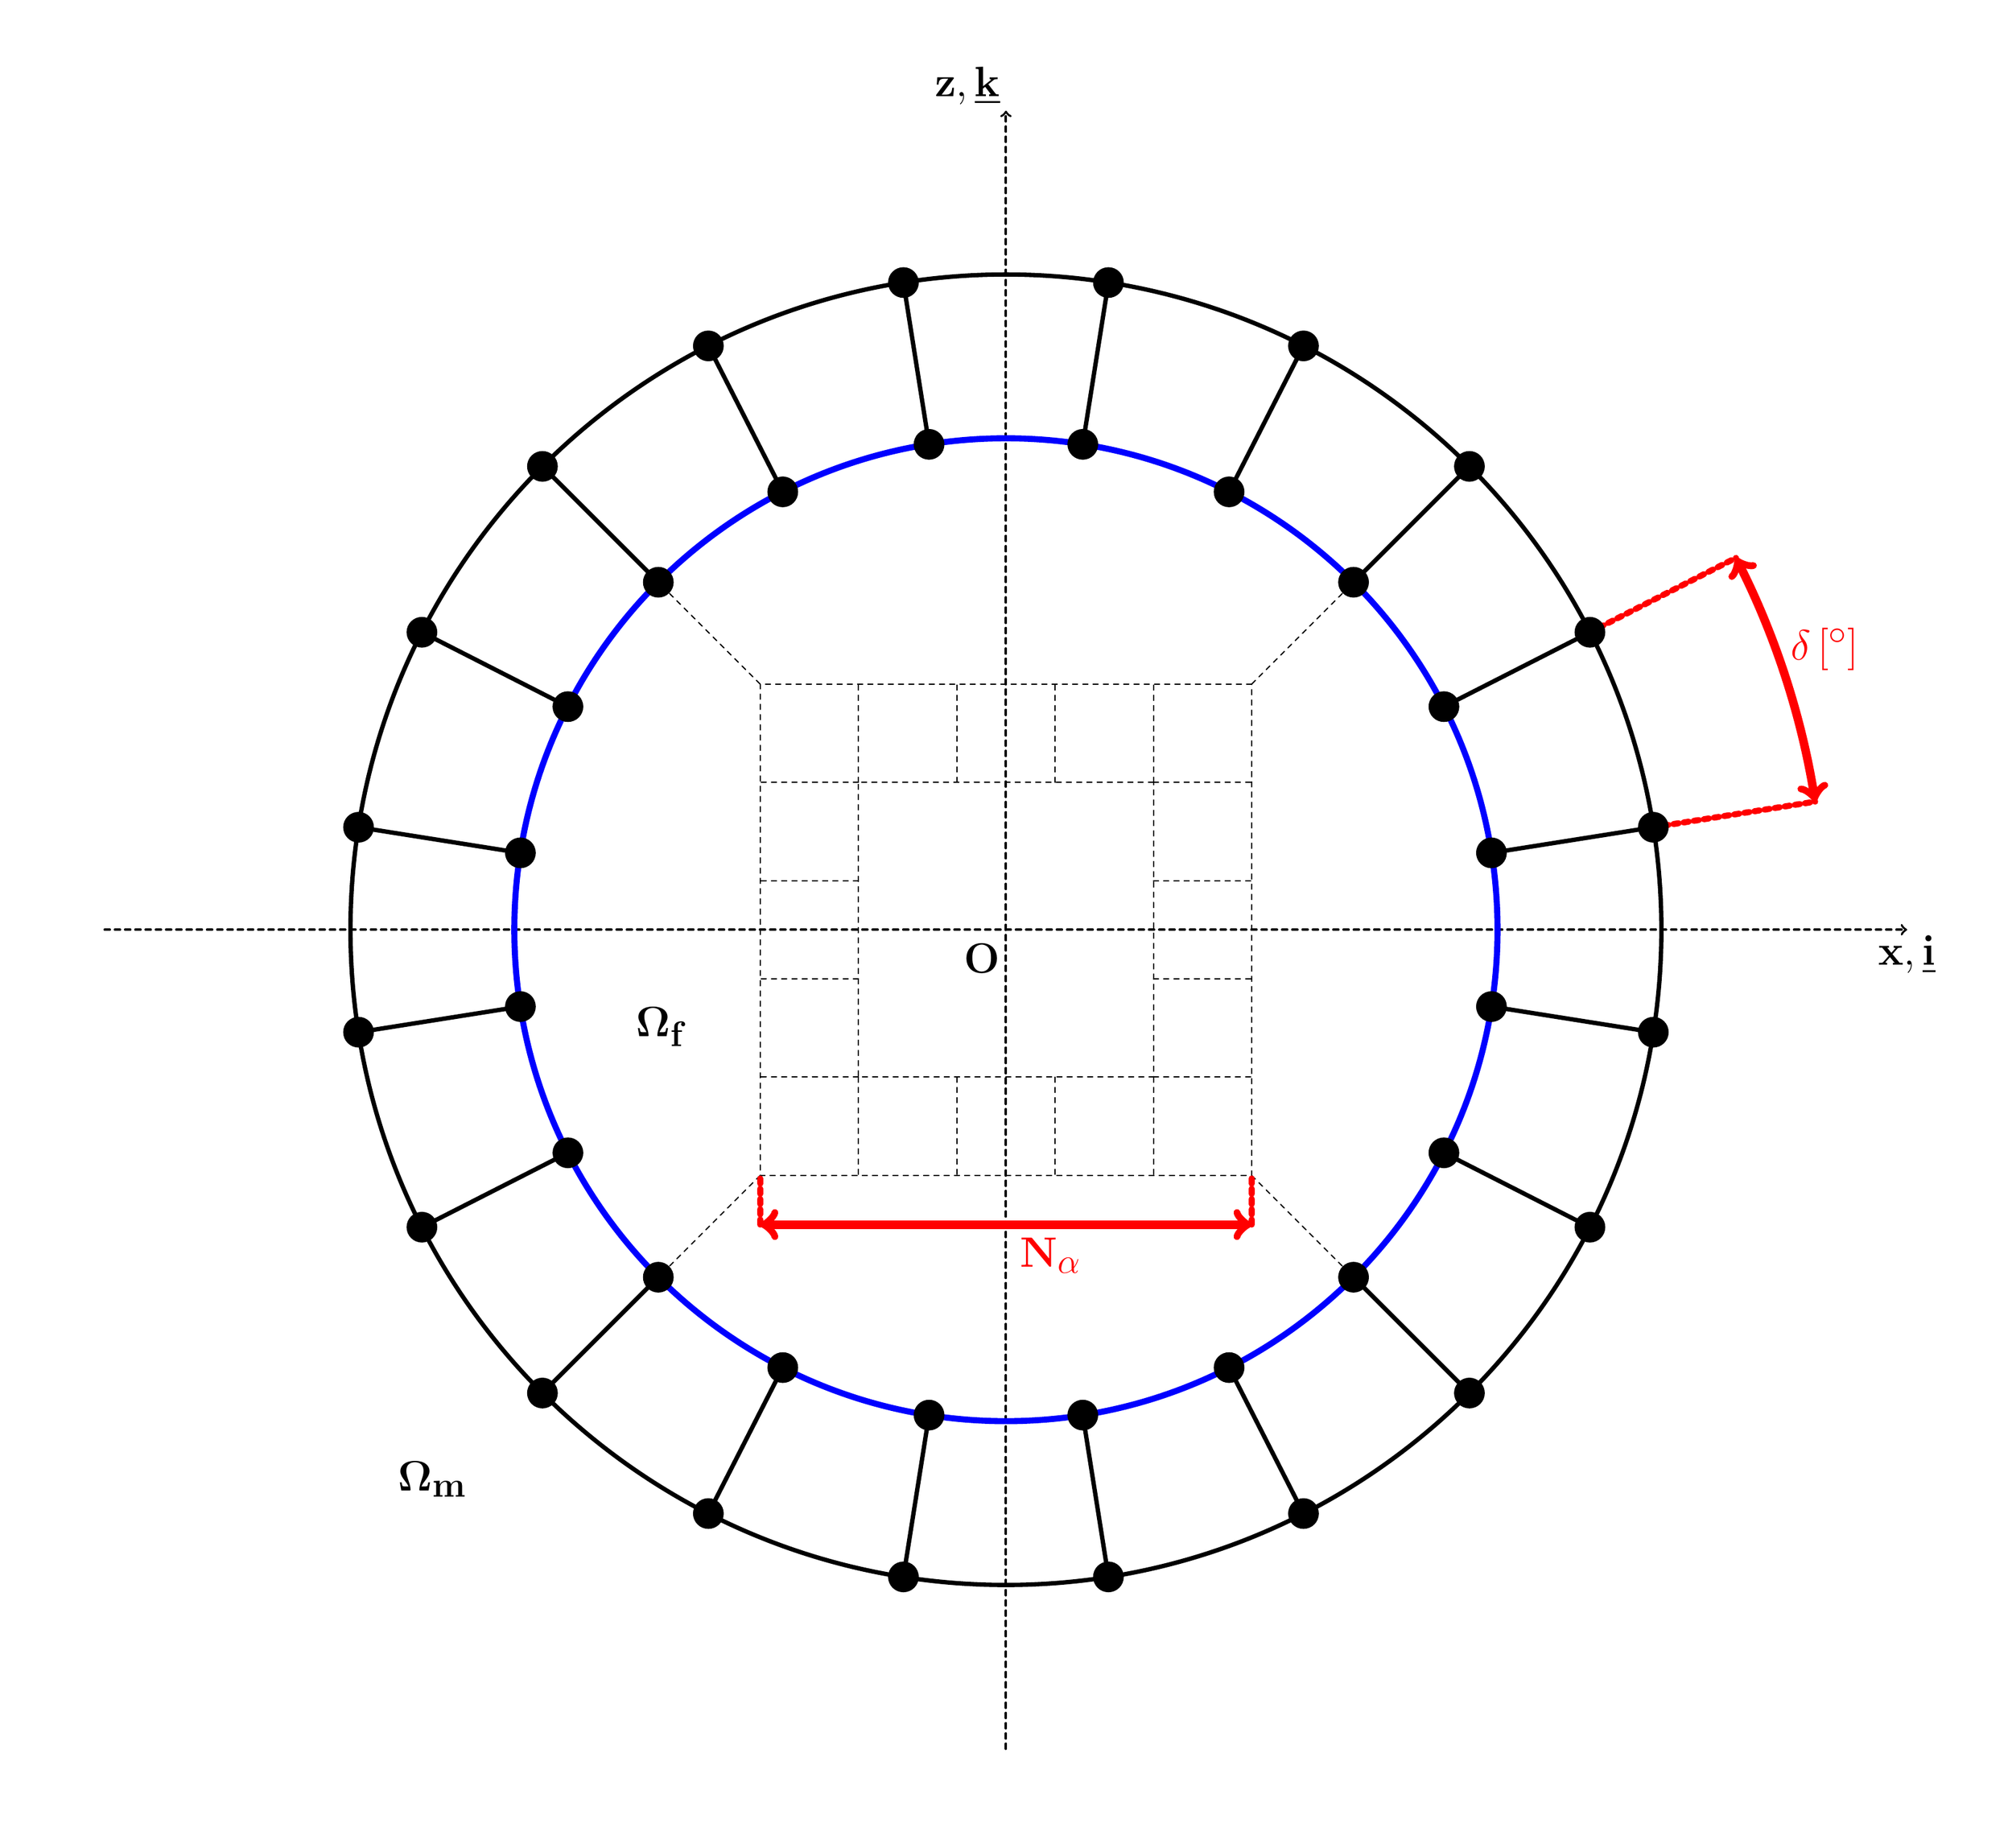
\begin{tikzpicture}[scale=4.5,cap=round,x=1.5cm,y=1.5cm]

%----------------------------------------------------------------------------------------------%
%                                                   CONSTANTS
%----------------------------------------------------------------------------------------------%

\def\pivalue{3.141592653589793238462643383279502884197169399375105820974944592307816406286}



\draw[->,dashed, line width = 0.5mm] (-2.75,0) -- (2.75,0);
\node[anchor=north] at (2.75,0) {\Huge $\mathbf{x,\underline{i}}$};
\draw[->,dashed, line width = 0.5mm] (0,-2.5) -- (0,2.5) ;
\node[anchor=south east] at (0,2.5) {\Huge $\mathbf{z,\underline{k}}$};
\node[text=black,anchor=north east] at (0,-0.025) {\Huge $\mathbf{O}$};

\draw[draw=blue, line width=1.25mm] (1.5,0)arc(0:360:1.5);
\draw[draw=black, line width=0.9mm] (2,0)arc(0:360:2);

\draw (-0.7*1.5,-0.25*1.5) node[black,above] {\Huge $\mathbf{\Omega_{f}}$};
\draw (-0.7*2.5,-0.7*2.5) node[black,above] {\Huge $\mathbf{\Omega_{m}}$};

\pgfmathsetmacro\costhetalow{cos(45+0.9*360)}
\pgfmathsetmacro\sinthetalow{sin(45+0.9*360)}
\pgfmathsetmacro\costhetamid{cos(45+0.925*360)}
\pgfmathsetmacro\sinthetamid{sin(45+0.925*360)}
\pgfmathsetmacro\costhetaup{cos(45+0.95*360)}
\pgfmathsetmacro\sinthetaup{sin(45+0.95*360)}
\draw[<->,draw=red, line width=1.75mm] (2.5*\costhetalow,2.5*\sinthetalow)arc(0.5*0.05*360:1.5*0.05*360:2.5);
\draw[draw=red, dashed, line width=1.25mm] (2*\costhetalow,2*\sinthetalow) -- (2.5*\costhetalow,2.5*\sinthetalow);
\draw[draw=red, dashed, line width=1.25mm]  (2*\costhetaup,2*\sinthetaup) -- (2.5*\costhetaup,2.5*\sinthetaup);
\node[text=red,anchor=south west] at (2.5*\costhetamid,2.5*\sinthetamid) {\Huge $\mathbf{\delta\left[^{\circ}\right]}$};

\foreach \n in{0,0.05,0.1,0.15,0.2,0.25,0.3,0.35,0.4,0.45,0.5,0.55,0.6,0.65,0.7,0.75,0.8,0.85,0.9,0.95}{
	\pgfmathsetmacro\costheta{cos(45+\n*360)}
	\pgfmathsetmacro\sintheta{sin(45+\n*360)}
	\draw[draw=black, line width=0.9mm] (1.5*\costheta,1.5*\sintheta) -- (2*\costheta,2*\sintheta);
	\fill (1.5*\costheta,1.5*\sintheta)  circle[radius=2pt];
	\fill (2*\costheta,2*\sintheta)  circle[radius=2pt];
}

\pgfmathsetmacro\sqrtTwo{sqrt(2)}

\foreach \n in{0,0.25,0.5,0.75}{
	\pgfmathsetmacro\costheta{cos(45+\n*360)}
	\pgfmathsetmacro\sintheta{sin(45+\n*360)}
	\draw[draw=black,dashed, line width=0.25mm] (0.75*\sqrtTwo*\costheta,0.75*\sqrtTwo*\sintheta)--(1.5*\costheta,1.5*\sintheta);

}

\foreach \n in{0.75}{
	\draw[draw=black,dashed, line width=0.25mm] (\n,\n) -- (-\n,\n) -- (-\n,-\n) -- (\n,-\n) -- (\n,\n);
	\pgfmathsetmacro\deltax{(2*\n)/5}
	\draw[draw=black,dashed, line width=0.25mm] (\n-\deltax,\n-\deltax) -- (-\n+\deltax,\n-\deltax) -- (-\n+\deltax,-\n+\deltax) -- (\n-\deltax,-\n+\deltax) -- (\n-\deltax,\n-\deltax);
	\foreach \m in{0,1,2,3}{
		\draw[draw=black,dashed, line width=0.25mm](-\n+\deltax+\m*\deltax,\n-\deltax)--(-\n+\deltax+\m*\deltax,\n);
		\draw[draw=black,dashed, line width=0.25mm](-\n+\deltax+\m*\deltax,-\n+\deltax)--(-\n+\deltax+\m*\deltax,-\n);
		\draw[draw=black,dashed, line width=0.25mm](\n-\deltax,-\n+\deltax+\m*\deltax)--(\n,-\n+\deltax+\m*\deltax);
		\draw[draw=black,dashed, line width=0.25mm](-\n+\deltax,-\n+\deltax+\m*\deltax)--(-\n,-\n+\deltax+\m*\deltax);
	}
}

\def\n{0.75}
\pgfmathsetmacro\deltax{(2*\n)/5}
\draw[<->,draw=red, line width=1.75mm] (\n,-\n-0.5*\deltax) -- (-\n,-\n-0.5*\deltax);
\draw[draw=red, dashed, line width=1.25mm] (-\n,-\n-0.5*\deltax) -- (-\n,-\n);
\draw[draw=red, dashed, line width=1.25mm]  (\n,-\n-0.5*\deltax) -- (\n,-\n);
\node[text=red,anchor=north west] at (0.025,-\n-0.575*\deltax) {\Huge $\mathbf{N_{\alpha}}$};

\node[anchor=south] at (0,2.75) {};
\node[anchor=south] at (0,-2.75) {};
\node[anchor=north] at (3,0) {};
\node[anchor=north] at (-3,0) {};




\end{tikzpicture}

\end{document}